\documentclass[12pt]{standalone}

\usepackage{tikz}
\usepackage{ctex}

\begin{document}
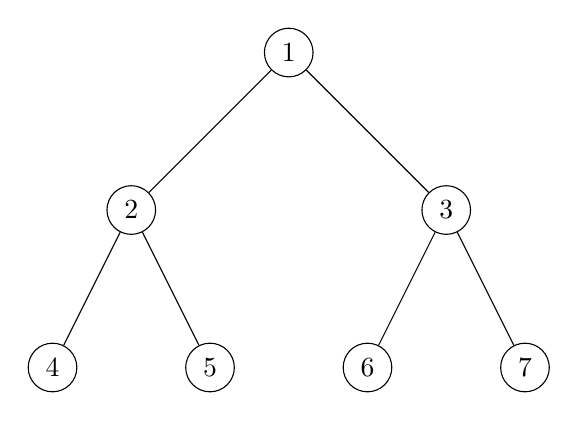
\begin{tikzpicture}
    [level distance=2cm,
    level 1/.style={sibling distance=4cm},
    level 2/.style={sibling distance=2cm}]

    \scoped[every node/.style={circle,draw}]
    \node (A) at (0,0) {$1$}
        child {node (B) {$2$}
            child {node (C) {$4$}}
            child {node (D) {$5$}}}
        child {node (E) {$3$}
            child {node (F) {$6$}}
            child {node (G) {$7$}}};

\end{tikzpicture}
\end{document}
